\documentclass[border=10pt]{standalone}
\usepackage{tikz}
\usetikzlibrary{arrows.meta, positioning, shapes.geometric, calc, fit, backgrounds, decorations.pathreplacing}
\usepackage{xcolor}

% ========== 颜色定义 ==========
% 修改这些来改变高亮状态
\definecolor{highlight}{RGB}{255, 100, 100}      % 当前工作模块(红色高亮)
\definecolor{completed}{RGB}{100, 200, 100}      % 已完成模块(绿色)
\definecolor{pending}{RGB}{200, 200, 200}        % 待完成模块(灰色)
\definecolor{inprogress}{RGB}{100, 150, 255}     % 进行中(蓝色)
\definecolor{dataflow}{RGB}{50, 50, 50}          % 数据流箭头

\begin{document}
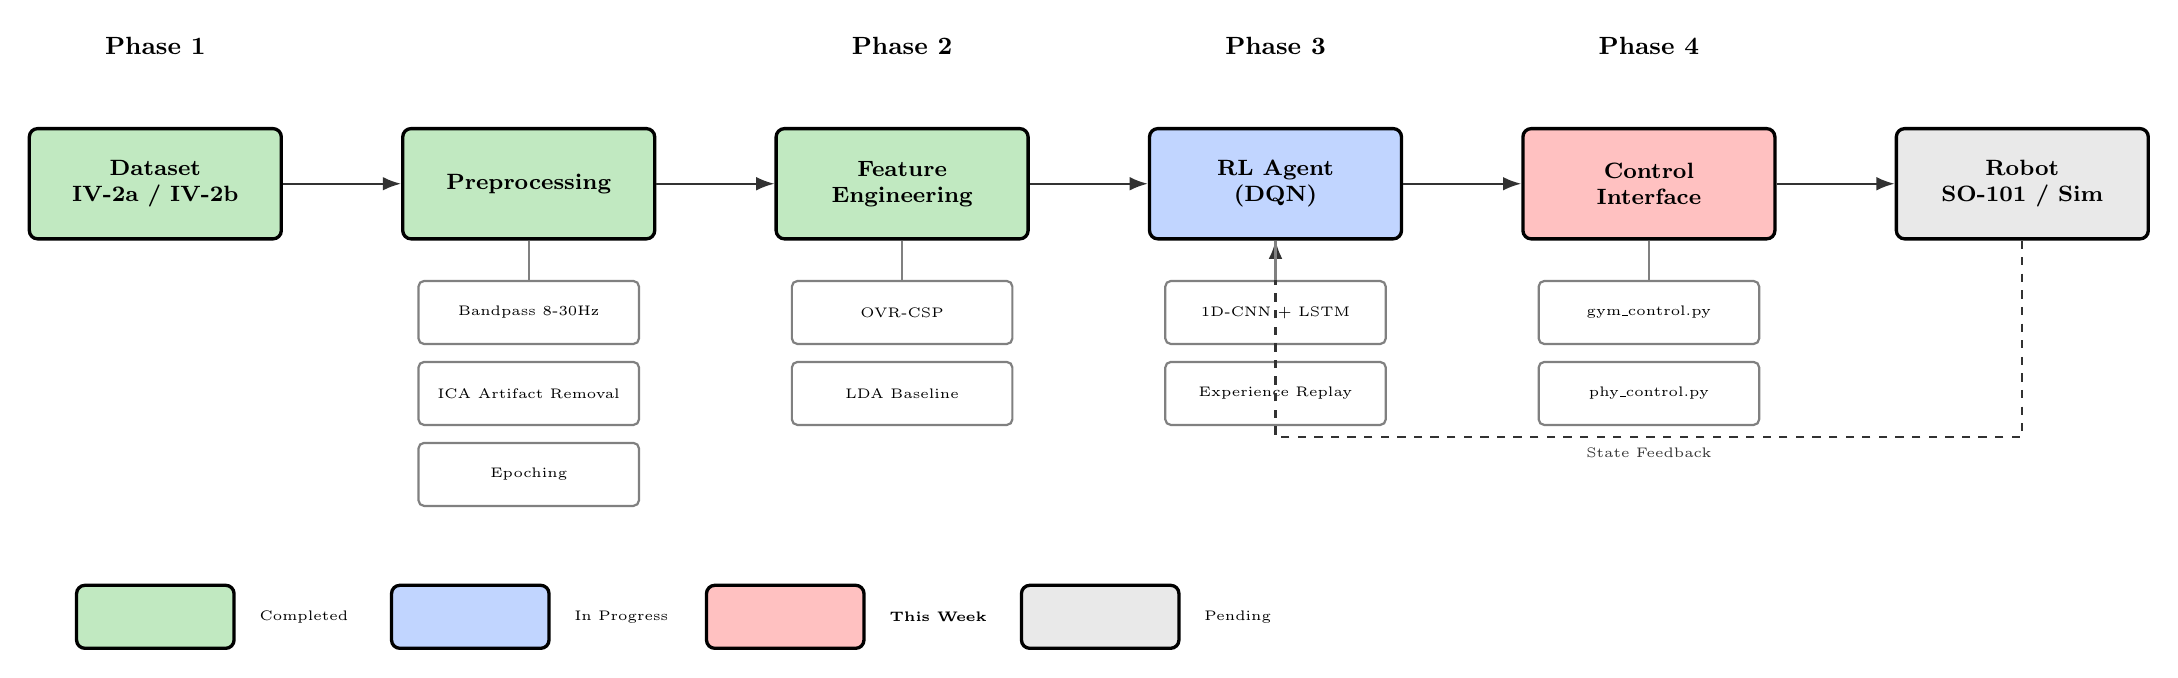
\begin{tikzpicture}[
    node distance=10mm and 15mm,
    % 模块样式
    module/.style={
        rectangle, rounded corners=3pt, draw=black, very thick,
        minimum width=32mm, minimum height=14mm,
        align=center, font=\footnotesize\bfseries
    },
    % 子模块样式
    submodule/.style={
        rectangle, rounded corners=2pt, draw=gray, thick,
        minimum width=28mm, minimum height=8mm,
        align=center, font=\tiny
    },
    % 箭头样式
    arrow/.style={-Latex, thick, dataflow},
    dashedarrow/.style={-Latex, thick, dashed, dataflow},
]

% ==================== 主要模块 ====================
% 修改 fill 颜色来改变每个模块的状态
% 选项: completed!40, inprogress!40, highlight!40, pending!40

% Phase 1: 数据采集与预处理
\node[module, fill=completed!40] (dataset) {Dataset\\IV-2a / IV-2b};

\node[module, fill=completed!40, right=of dataset] (preprocess) {Preprocessing};

% Phase 2: 特征工程
\node[module, fill=completed!40, right=of preprocess] (feature) {Feature\\Engineering};

% Phase 3: RL 训练
\node[module, fill=inprogress!40, right=of feature] (rl) {RL Agent\\(DQN)};

% Phase 4: 执行
\node[module, fill=highlight!40, right=of rl] (control) {Control\\Interface};

\node[module, fill=pending!40, right=of control] (robot) {Robot\\SO-101 / Sim};

% ==================== 子模块(可选) ====================
\node[submodule, below=5mm of preprocess] (filter) {Bandpass 8-30Hz};
\node[submodule, below=2mm of filter] (ica) {ICA Artifact Removal};
\node[submodule, below=2mm of ica] (epoch) {Epoching};

\node[submodule, below=5mm of feature] (csp) {OVR-CSP};
\node[submodule, below=2mm of csp] (lda) {LDA Baseline};

\node[submodule, below=5mm of rl] (qnet) {1D-CNN + LSTM};
\node[submodule, below=2mm of qnet] (replay) {Experience Replay};

\node[submodule, below=5mm of control] (gym) {gym\_control.py};
\node[submodule, below=2mm of gym] (phy) {phy\_control.py};

% ==================== 数据流箭头 ====================
\draw[arrow] (dataset) -- (preprocess);
\draw[arrow] (preprocess) -- (feature);
\draw[arrow] (feature) -- (rl);
\draw[arrow] (rl) -- (control);
\draw[arrow] (control) -- (robot);

% 反馈回路
\draw[dashedarrow] (robot.south) -- ++(0,-25mm) -| node[pos=0.25, below, font=\tiny] {State Feedback} (rl.south);

% 子模块连接线
\draw[gray, thick] (preprocess.south) -- (filter.north);
\draw[gray, thick] (feature.south) -- (csp.north);
\draw[gray, thick] (rl.south) -- (qnet.north);
\draw[gray, thick] (control.south) -- (gym.north);

% ==================== Phase 标签 ====================
\node[above=8mm of dataset, font=\small\bfseries] {Phase 1};
\node[above=8mm of feature, font=\small\bfseries] {Phase 2};
\node[above=8mm of rl, font=\small\bfseries] {Phase 3};
\node[above=8mm of control, font=\small\bfseries] {Phase 4};

% ==================== 图例 ====================
\begin{scope}[shift={(0,-55mm)}]
    \node[module, fill=completed!40, minimum width=20mm, minimum height=8mm] at (0,0) {};
    \node[right, font=\tiny] at (12mm, 0) {Completed};
    
    \node[module, fill=inprogress!40, minimum width=20mm, minimum height=8mm] at (40mm,0) {};
    \node[right, font=\tiny] at (52mm, 0) {In Progress};
    
    \node[module, fill=highlight!40, minimum width=20mm, minimum height=8mm] at (80mm,0) {};
    \node[right, font=\tiny] at (92mm, 0) {\textbf{This Week}};
    
    \node[module, fill=pending!40, minimum width=20mm, minimum height=8mm] at (120mm,0) {};
    \node[right, font=\tiny] at (132mm, 0) {Pending};
\end{scope}

\end{tikzpicture}
\end{document}

